% Результаты анализа
\chapter{Исследование свойств прототипа системы считывания и сбора данных детектора CBM RICH}\label{sec:secAnalysisResults}

% \todo Добавить в текст из диссера копфера картинку 4.8 со страницы 72

\begin{figure}[H]
\centering
\includegraphics[width=0.6\textwidth]{pictures/QEcurvesKopfer.png}
\caption{}
\label{fig:QEcurvesKopfer}
\end{figure}

% Ну вот картинка тут, но куда-то надо её подвинуть.

\subsection{Испытание системы сбора данных с использованием FLIB}\label{section:flib}

Значительная часть данных была набрана параллельно двумя системами сбора данных. Было проведено побайтное сравнение результатов распаковки обоих потоков. На массиве составляющем примерно $ 10^{?} $ сообщений расхождений не выявлено. Таким образом, продемонстрирована работоспособность концепции формирования временных интервалов и ввода данных в компьютер с использованием FLIB. Приведённые в следующих разделах результаты получены на основе данных, записанных с использованием DABC.
\section{LeadingEdgeDiff}\label{sec:secLeadingEdgeDiff}

Один из этапов обработки данных --- построение событий. В данной работе рассматривается два типа событий --- сигналы от лазера и сигналы от черенковского кольца. В любом случае, событие --- это структура данных, содержащая информацию о хитах, сгруппированных по времени. Каждый хит содержит, как минимум, временную отметку момента прихода переднего фронта сигнала и номер канала, который в случае CBM~RICH указывает номер пикселя фоточувствительной камеры, т.е. говорит о геометрическом положений зарегистрированного фотона.

Данное исследование посвящено, в первую очередь, временным характеристикам системы считывания, поэтому в основном речь пойдёт о временных отметках.

Очевидно, что для каждого события можно построить несколько распределений, которые на большом массиве данных, т.е. на многих событиях, характеризуют систему считывания и могут быть использованы для калибровки электроники с целью повышения временного разрешения системы. Т.к. событие имеет максимальную ширину, определяемую размерами окна в алгоритме построения событий, распределения могут иметь ``обрезанные хвосты'', которые, однако, невозможно избежать.

Пусть событие содержит N хитов. Введём внутри события нумерацию хитов от 0 до N. Пусть внутри события хиты упорядочены по времени, т.е. хит с временной отметкой $ t_{0} $ был зарегистрирован раньше остальных, а хит с временной отметкой $ t_{N} $ --- позже всех. Такой порядок может, например, обеспечиваться естественным образом алгоритмом построения событий. Внутри события все временные отметки зарегистрированы в разных каналах --- множественные хиты в одном канале в одном событий являются признаком того, что порог дискриминатора установлен слишком низко и регистрируются шумы. Введём в рассмотрение распределение $ \omega $ разностей временных отметок всех хитов, кроме первого, относительно первого, т.е. распределение

{\centering
$ t_{j} - t_{0} $, где  $ j \in [1..N] $.\\
}

Также введём распределение $ \sigma_{1} $ всех пар временных отметок одного события, т.е.

{\centering
$ t_{j}-t_{i} $, где $ i \in [0..N], j \in [0..N], i \neq j $.\\
}

Очевидно, что в такой формулировке одна и та же пара временных отметок войдёт в распределение дважды с разными знаками --- например, $ t_{1}-t_{2} $ и $ t_{2}-t_{1} = -(t_{1}-t_{2}) $. Это делает распределение симметричным, среднее значение строго равно 0, а ширина распределения чуть больше, чем в случае, когда нет дублирования информации. Введём непрерывную нумерацию каналов и примем, что в разности $ t_{j}-t_{i} $ первая временная отметка была зарегистрирована каналом $a$, а вторая --- каналом $b$. Введём распределение $ \sigma_{2} $, по сути очень похожее на $ \sigma_{1} $, но без дублирования информации, в котором будем учитывать только пары, у которых $ b > a $.

В идеальной ситуации, если событие соответствует одной вспышке лазера или одному черенковскому кольцу, и отсутствуют факторы, размывающие время регистрации, все разницы были бы равны нулю. В качестве таких размывающих факторов можно привести, например, следующие: временные характеристики лазера, разброс геометрических путей черенковских фотонов, разброс времени прохождения электронной лавины в динодной системе ФЭУ, дребезг сигналов в передней электронике. Из-за перечисленных явлений распределение $ \omega $ имеет следующую форму --- (описание). Распределение $ \sigma_{2} $ --- (описание).

%Распределение $ \sigma_{2} $ позволяет определить относительную задержку распространения сигнала,
%Влияние всех этих явлений выливается в то, что распределение $ \sigma $ имеет колоколообразную форму.

Среднее значение либо положение масимума распределения $ \sigma_{2} $ можно использовать для того, чтобы определить значение поправки для данной пары каналов. Если выполнить анализ с применением коррекций, то вид всех распределений изменится. $ \omega $ сгруппируется ближе к нулю, $ \sigma_{2} $ передвинется к нулю, а $ \sigma_{1} $ сузится к нулю.

Представляется возможность анализировать различные области фоточувствительной камеры. Интересно группировать хиты в соответствии с тем, какой электроникой они обрабатываются. В данном анализе было введено 4 подмножества: 1~пара каналов, 16~каналов одной платы передней электроники, 64~канала одного МА~ФЭУ, 256~каналов 4~МА~ФЭУ, образующих площадку 2х2~МА~ФЭУ в одном углу камеры. При том, что вся фоточувствительная камера на пучковых тестах имела размер 4х4~МА~ФЭУ, рассматривать более 4~МА~ФЭУ одновременно не имеет смысла, т.к. в прототипе были установлены различные модели МА~ФЭУ, некоторые покрытые сместителем спектра, а некоторые нет.

\subsection{Калибровка точного времени (Fine time calibration)}\label{section:FTcalib}

Пример таблицы калибровки точного времени, полученной на данных лабораторных тестов, представлен в виде графика на рисунке \ref{fig:TypicalCalibTable}. По оси абсцисс откладывается значение счётчика точного времени, а по оси ординат --- значение точного времени в наносекундах. Вид графика не зависит от того, по каким данным он был построен, так как он определяется архитектурой время-цифрового преобразователя. Обратим внимание, что в диапазоне значений десятибитного счетчика точного времени интервалу равному периоду грубого счетчика, т.е. 5~нс, соответствуют отсчеты от 30 до 520. Точные границы интервала определяются тем, что значения задержек отдельных элементов цифровой линии задержки индивидуальны и зависят от флуктуаций технологического процесса.
%Было: Точные границы интервала определяются тем, что задержки на каждой ступени индивидуальны и зависят от флуктуаций технологического процесса.
% хотя бы - на каждом элементе

С целью понимания особенностей работы счетчиков точного времени, каждая таблица калибровки точного времени была аппроксимирована кусочно-линейной функцией. На рисунке \ref{fig:CalibTableMinusFit} показан пример разности значений функции калибровки точного времени и линейной функции. Видно, что отклонения не превышают 60 пс.
% фитирована - аппроксимирована

% Макросы для получения этих картинок лежат в Data_analysis_repo/threshold_scan_2/
\begin{figure}
\includegraphics[width=1.0\textwidth]{pictures/CalTable_0010_01.eps}
\caption{Пример калибровочной кривой.}
\label{fig:TypicalCalibTable}
\end{figure}

% Макросы для получения этих картинок лежат в Data_analysis_repo/threshold_scan_2/
\begin{figure}
\includegraphics[width=1.0\textwidth]{pictures/CalTableMinusFit_0010_01.eps}
\caption{Отклонение калибровочной кривой от линейной функции.}
\label{fig:CalibTableMinusFit}
\end{figure}

Каждая аппроксимирующая кусочно-линейная функция состоит из трёх отрезков и может быть однозначно описана двумя координатами изломов, которые приблизительно соответствуют двум крайним рабочим значениям счётчика точного времени. Параметры линейных функций для всех каналов отображены на двумерной гистограмме на рисунке \ref{fig:ABmap}.
% строго говоря, это не гистограмма (диаграмма?)
Видно, что распределение хотя и двугорбое, но достаточно компактное.

Один из возможных способов оценки влияния калибровки на точность регистрации временных отметок это исследование физически одновременных фронтов, которые можно получить, например, с помощью высокоточного генератора прямоугольных импульсов.

%Влияние замены точной функции калибровки на приближенную можно увидеть при одновременной оцифровке на нескольких каналах ВЦП сигналов с высокоточного генератора прямоугольных импульсов.
%(Сначала нужно сказать, что для оценки качества калибровки необходимо исследовать одновременные фронты, которые можно получить от высокоточного генератора прямоугольных импульсов.)
%(Расписать подробно ряд: точная калибр., индивид. линейная функция, глоб линейная функция, отсутствии калибр.)

В процедуре калибровки для каждого канала была выполнена замена калибровочной таблицы сначала индивидуальной линейной функцией данного канала, а потом усредненной. Полученные распределения измеренной ширины импульса в исследуемом канале показаны на рисунке \ref{fig:FourToT}.

% Значение 30 пс я получил из распределения по передним фронтам, FWHM в линейной шкале. Это среднее знечение по нескольким каналам. Разброс очень маленький.
% При использовании индивидуальной калибровки получается 70 пс.
% А вот сравнивать это со случаями без калибровки или с усреднённой калибровкой не очень корретно, потому что вид распределения двухпиковый и ширина одного пика лишь немного больше, но воторой пик оказывает своё влияние.
Видно, что полноценная калибровка точного времени необходима для достижения предельной точности ВЦП, составляющей 30~пс (FWHM). Использование индивидуальной линейной функции приводит к падению точности до 70~пс, а усреднённой --- до ??? (без калибровки) в наиболее неблагоприятных каналах.
Таким образом, при невозможности выполнить калибровку точного времени, например, из-за недостаточного массива данных, предоставленных для анализа, в условиях нашей задачи, когда характерное временное разрешение составляет несколько сотен пикосекунд, возможно применение усредненной линейной функции без заметного снижения точности.

% Макросы для получения этих картинок лежат в Analysis_Sep2016/WLS_off/calibration_files/
\begin{figure}
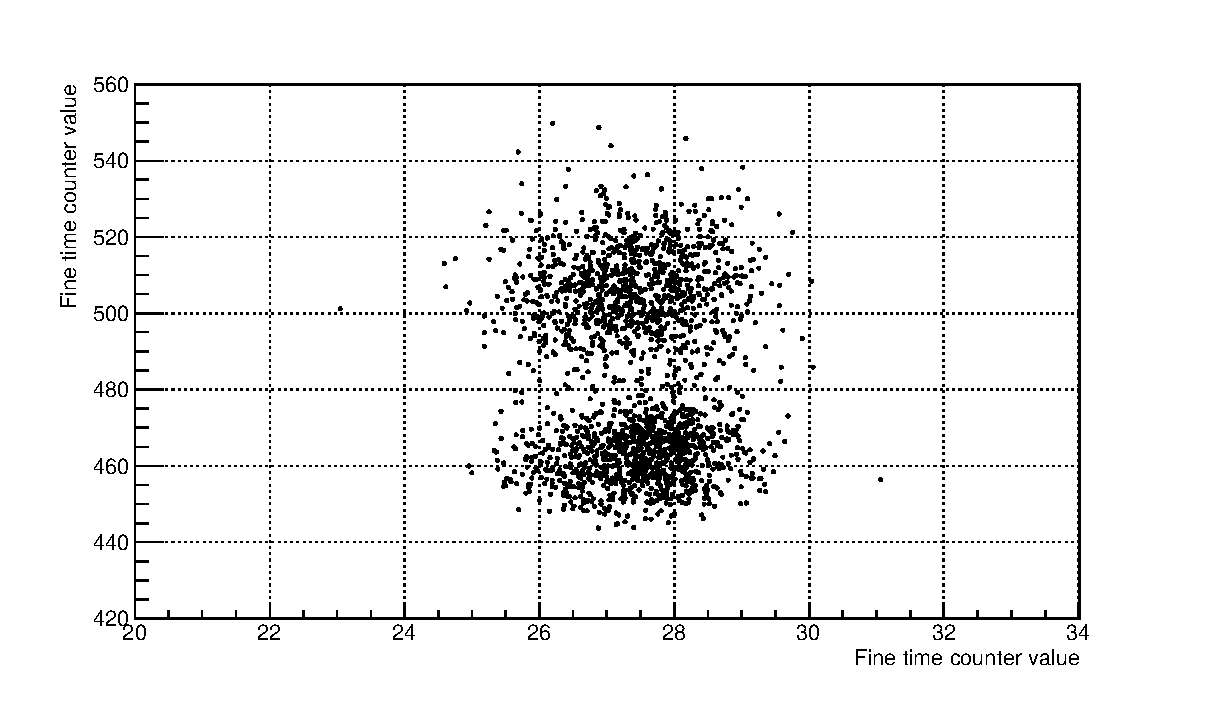
\includegraphics[width=1.0\textwidth]{pictures/ABmap.eps}
\caption{Распределение координат точек излома аппроксимирующих кусочно-линейных функций.}
% для большого набора каналов по данным с пучковых тестов
\label{fig:ABmap}
\end{figure}

% Макросы для получения этих картинок лежат в Data_analysis_repo/directTDC/
\begin{figure}
\includegraphics[width=1.0\textwidth]{pictures/ToT_ch2.eps}
\caption{Результаты измерения ширины импульса от генератора в случае: без калибровки точного времени; с применением усреднённой калибровочной фукнции; с применением индивидуальной линейной калибровочной функции; с применением полноценной калибровочной таблицы.}
\label{fig:FourToT}
\end{figure}

Приведённые выше функции калибровки были построены по массиву данных, содержащихся в семи файлах. Каждый файл это 2~минуты измерений при частоте генератора 5~кГц, т. е. около 600~тысяч вспышек лазера. Таким образом, всего было 4.2~миллиона вспышек за  14~минут, а один файл составляет приблизительно 15\%~от полного набора данных. В каждом канале было зарегистрировано от~300 до~400~тысяч временных отметок, которые были использованы для выполнения калибровки. Для иллюстрации стабильности калибровки на рисунке~\ref{fig:Stability} показана разность функций калибровки, построенных по всему массиву данных и функций, построенных на файлах, составляющих $ \approx $15\%~данных каждый, взятых в начале, середине и конце набора данных. Видно, что отклонения в основном не превышают 10~пс, однако имеются редкие выбросы до 20~пс.

\begin{figure}
\includegraphics[width=1.0\textwidth]{pictures/calibrationStability_dec2016.eps}
\caption{Стабильность калибровок.}
\label{fig:Stability}
\end{figure}

\subsection{Определение коррекций задержек между каналами}\label{section:Corrections}

Типичная гистограмма разности временных отметок передних фронтов, соответствующих фотонам из одной вспышки лазера, зарегистрированных в заданной паре каналов, показана на \figref{fig:TypicalLeadingEdgeDiff}. Такие гистограммы позволяют определить положение пика и, соответственно, ввести коррекцию задержки. Отметим, что наблюдается дрейф порядка 0.5~нс значений задержек, полученных таким образом, что даёт заметный вклад во временное разрешение системы считывания (см.~секцию~\ref{section:TimeRes}).

Наблюдается также аддитивность задержек, т.е. задержка в i-м канале относительно опорного может быть получена с точностью не хуже ??? пс как сумма задержки в j-м канале относительно опорного и задержки в i-м канала относительно j-го. Для некоторых пар каналов вид гистограммы отличается от показанной на \figref{fig:TypicalLeadingEdgeDiff}. См., например, \figref{fig:LeadingEdgeDiffMultiplePeaks}. Подобное распределение можно получить, если один из двух каналов является дефектным в том смысле, что к фронту логического сигнала подмешивается возбужденный или наведённый колебательный сигнал. Такая гипотеза подтверждается тем фактом, что форма гистограммы зависит от порога дискриминатора на плате PADIWA. При построении аналогичной гистограммы для пары дефектных каналов наблюдается до 5~пиков. Дальнейшее исследование проводилось с исключением дефектных каналов. Доля дефектных каналов составляет около 10\% от полного числа каналов. При разработке следующей версии передней электроники для CBM RICH особое внимание будет уделено электромагнитной чистоте каналов, а гистограммы подобные обсуждаемым в данном разделе будут использоваться в качестве диагностического инструмента.

% не нужно обособить запятыми "подобные обсуждаемым в данном разделе"?

\begin{figure}
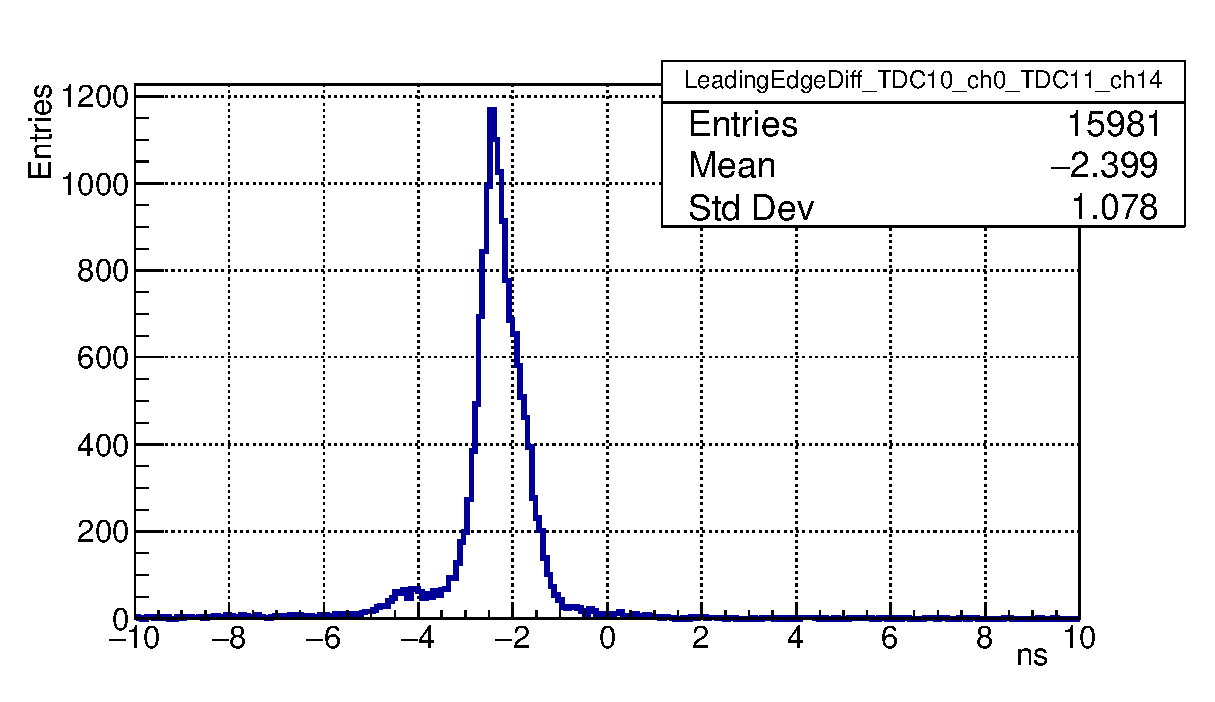
\includegraphics[width=1.0\textwidth]{pictures/22_LeadingEdgeDiff_TDC10_ch0_TDC11_ch14_feb2017.eps}
\caption{Распределение разности временных отметок передних фронтов, соответствующих фотонам из одной вспышки лазера, зарегистрированных в заданной паре каналов.}
\label{fig:TypicalLeadingEdgeDiff}
\end{figure}

\begin{figure}
\begin{minipage}[b]{0.495\textwidth}
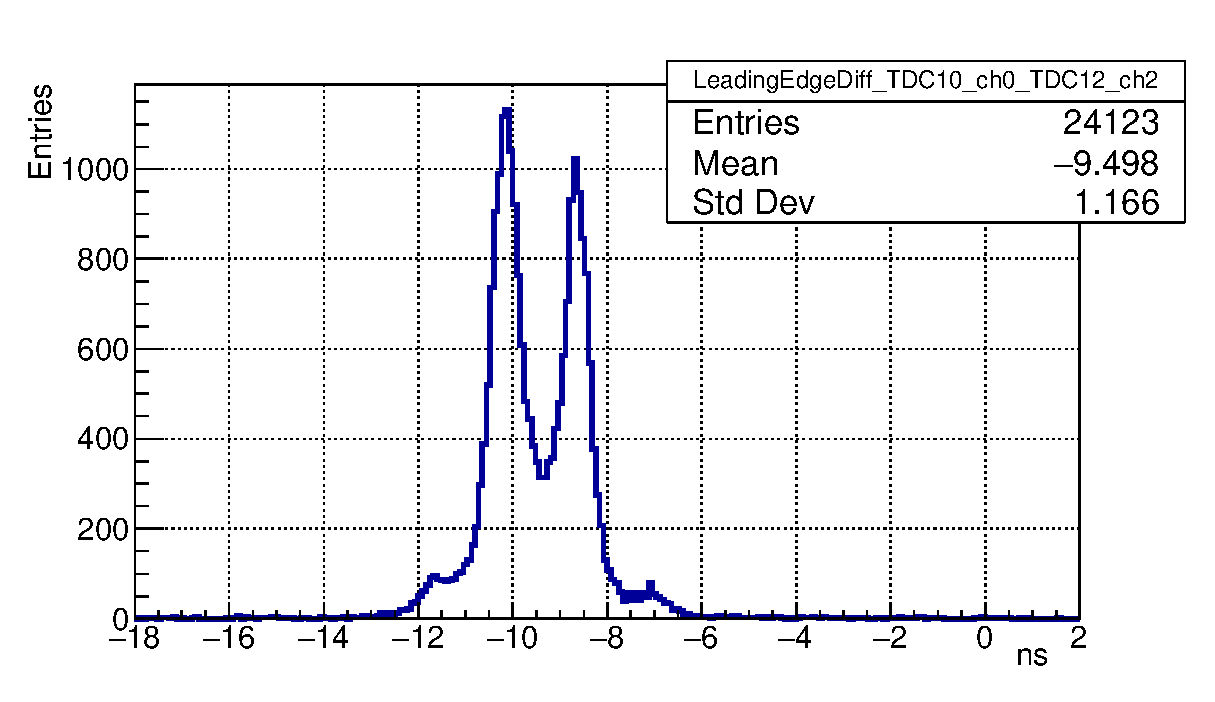
\includegraphics[width=1.0\textwidth]{pictures/23_LeadingEdgeDiff_TDC10_ch0_TDC12_ch2_feb2017.eps}
\end{minipage}
\hspace{0.01\textwidth}
\begin{minipage}[b]{0.495\textwidth}
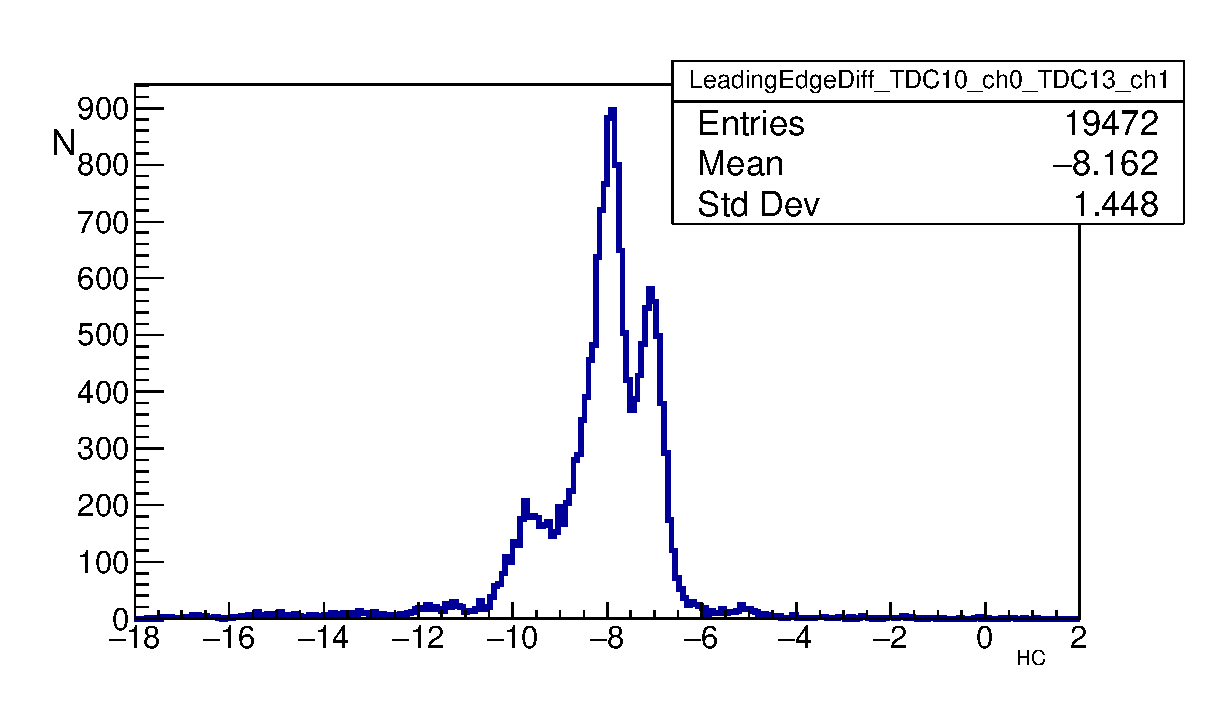
\includegraphics[width=1.0\textwidth]{pictures/23_LeadingEdgeDiff_TDC10_ch0_TDC13_ch1_feb2017.eps}
\end{minipage}
\caption{Распределение разности временных отметок передних фронтов, соответствующих фотонам из одной вспышки лазера, зарегистрированных в заданной паре каналов, при условии, что один из каналов --- дефектный.}
\label{fig:LeadingEdgeDiffMultiplePeaks}
\end{figure}

%\begin{figure}
%\includegraphics[width=1.0\textwidth]{pictures/}
%\caption{}
%\label{fig:}
%\end{figure}
\subsection{Временное разрешение}\label{section:TimeRes}

В проведённых пучковых тестах имеют место два типа событий, в которых регистрируются несколько практически одновременно испущенных фотонов. Первый тип --- это вспышка лазера, длительность которой на порядок меньше разброса времени прохождения сигнала через МА~ФЭУ. Второй тип --- черенковские кольца.
%В обоих случаях! Не так ли?
В этом случае разброс времени прихода фотонов на МА~ФЭУ может достигать 100~пс и определяется в первую очередь наклоном плоскости в которой расположены фотокатоды. Анализ таких событий позволяет охарактеризовать временное разрешение всей системы считывания, начиная от окна МА~ФЭУ и кончая формированием отметок времени. Временное разрешение одного канала определяется разбросом зарегистрированных временных отметок относительно времени прилёта фотона при многократных измерениях. Поскольку точное время прилёта фотона измерить нельзя, нам приходится исследовать разброс разностей временных отметок в паре каналов при регистрации одновременно пришедших фотонов. Временные отметки в каждом из каналов подвержены независимым флуктуациям по одинаковому закону, следовательно, измеренная ширина распределения будет в~$\sqrt 2$~раз больше, чем временное разрешение каждого канала. На рис.~\ref{fig:TimeRes} показано типичное распределение разностей временных отметок, принадлежащих одной вспышке лазера, после применения коррекций задержек и калибровки точного времени в двух каналах, ни один из которых не является дефектным.

\begin{figure}
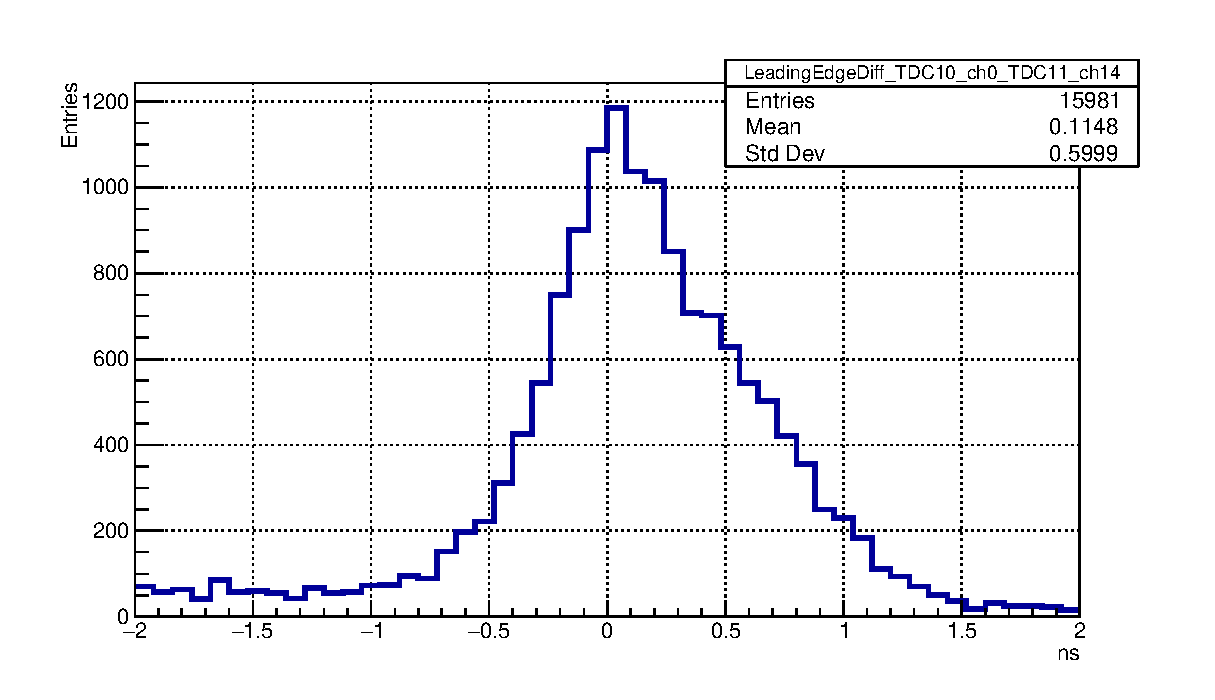
\includegraphics[width=1.0\textwidth]{pictures/LeadingEdgeDiff_TDC10_ch0_TDC11_ch14_corr.eps}
\caption{Распределение разности временных отметок передних фронтов, соответствующих фотонам из одной вспышки лазера, зарегистрированных в заданной паре каналов, после применения калибровки точного времени и коррекции задержек.}
\label{fig:TimeRes}
\end{figure}

Полная ширина на полувысоте (FWHM) этого распределения составляет 750~пс, что соответствует временному разрешению 530~пс. Данное значение превосходит разброс времён прохождения сигнала в МА~ФЭУ примерно в 2~раза. Причина расхождения заключается в отсутствии коррекции момента пересечения порога в зависимости от амплитуды сигнала. Для реализации такой коррекции необходимо надёжное измерение времени над порогом, что в нашем случае невозможно, см.~секцию~\ref{section:secToT}.

Для того чтобы охарактеризовать временное разрешение системы в целом, помимо анализа пар каналов исследовались физически одновременные сигналы на следующих совокупностях каналов: (1)~шестнадцать каналов, считываемых одной платой PADIWA, (2)~64~канала, принадлежащих одному МА~ФЭУ, (3)~256~каналов, принадлежащих четырём соседним МА~ФЭУ. В каждом случае после коррекции задержек и калибровки точного времени, отбирались все хиты, принадлежащие одному событию, и гистограммировались разности временных отметок по всем возможным парам каналов. Результаты для вспышек лазера показаны на рис.~\ref{fig:TimeResEvolutionLaser}. В таблице~\ref{tabl:EvolutionParams} показано, как эволюционирует среднеквадратичное отклонение и FWHM в зависимости от числа каналов.
% выкинул "полная ширина на полувысоте", т.к. ввёл сокращение выше
Отметим, что среднеквадратичное отклонение меняется слабо, а FWHM возрастает с увеличением числа каналов, одновременно с тем, что распределение последовательно принимает форму, более близкую к распределению Гаусса. Такое поведение можно интерпретировать как размывание индивидуальных особенностей каналов в процессе усреднения. Аналогичное поведение наблюдается и для хитов, принадлежащих одному черенковскому кольцу, см. рис.~\ref{fig:TimeResEvolutionRings}.

\begin{figure}
\includegraphics[width=1.0\textwidth]{pictures/TimePrecision_evolution_laser.eps}
\caption{Распределения для четырёх различных наборов каналов для событий от лазера.}
\label{fig:TimeResEvolutionLaser}
\end{figure}

\begin{figure}
\includegraphics[width=1.0\textwidth]{pictures/TimePrecision_evolution_rings.eps}
\caption{Распределения для четырёх различных наборов каналов для событий от черенковских колец.}
\label{fig:TimeResEvolutionRings}
\end{figure}

\begin{table}[h]
\caption{FWHM и RMS распределений при различных наборах исследуемых каналов.}
\label{tabl:EvolutionParams}
\begin{tabular}{ | p{0.34\linewidth} | p{0.15\linewidth} | p{0.15\linewidth} | p{0.15\linewidth} | p{0.15\linewidth} | }
	\hline
	Анализируемая область & Пара каналов & Плата PADIWA & Один МА~ФЭУ & Четыре МА~ФЭУ \\
	\hline
	Кол-во каналов & 2 & 16 & 64 & 256 \\
	\hline
	FWHM, лазер, нс & 1.1 & 1.2 & 1.5 & 1.7 \\
	\hline
	FWHM, кольца, нс & 0.6 & 0.8 & 1.0 & 1.3 \\
	\hline
	RMS, лазер, нс & 0.913 & 1.093 & 0.997 & 1.034 \\
	\hline
	RMS, кольца, нс & 1.238 & 1.379 & 1.430 & 1.487 \\
	\hline
\end{tabular}
\end{table}

\subsection{Исследование профиля высвечивания сместителя спектра}\label{section:secWLS}

Анализ распределения во времени хитов, принадлежащих одному черенковскому кольцу, позволяет исследовать временные свойства сместителя спектра. Анализу подлежит распределение разностей временных отметок хитов каждого кольца относительно первого по времени хита в данном кольце. В зависимости от длины волны черенковский фотон может с той или иной вероятностью либо поглотиться сместителем спектра и вызвать его свечение, либо пройти сквозь слой сместителя спектра без взаимодействия и попасть фотокатод. В результате, даже при наличии слоя сместителя спектра, часть хитов подчиняется временной зависимости характерной для чистого ФЭУ. Таким образом, для получения кривой высвечивания сместителя спектра необходимо из распределения разностей времен, полученного со сместителем спектра, вычесть должным образом отнормированное в максимуме распределение разностей времён, полученное с чистым ФЭУ.

Нормированные в максимуме кривые высвечивания со сместителем спектра и без него показаны на рис.~\ref{fig:WLStwoCurves}, а разность этих распределений --- на рисунке~\ref{fig:WLSdiff}. Видно, что за исключением небольшой выпуклости в области 7~нс, связанной с особенностями работы данного семейства МА~ФЭУ, кривая выглядит похоже на сумму нескольких экспонент.

\begin{figure}
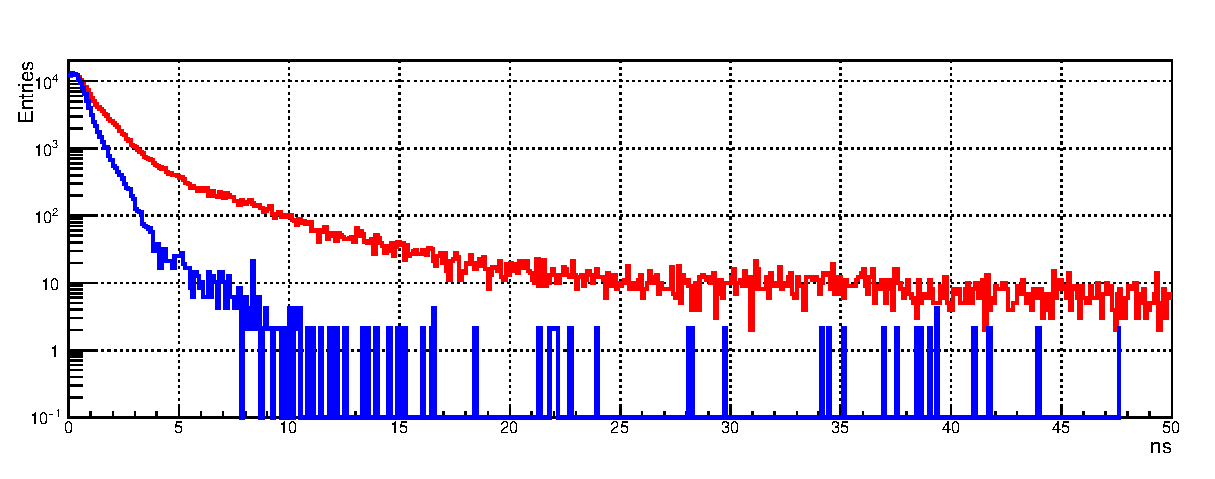
\includegraphics[width=1.0\textwidth]{pictures/WLS.eps}
\caption{Измеренные кривые высвечивания со сместителем спектра (красный, выше) и без него (синий, ниже).}
\label{fig:WLStwoCurves}
\end{figure}

\begin{figure}
\includegraphics[width=1.0\textwidth]{pictures/WLSdiff_1Nov.eps}
\caption{}
\label{fig:WLSdiff}
\end{figure}

Указанная выпуклость не позволяет надёжно извлечь характерные времена высвечивания. Интересно, тем не менее, сравнить полученную кривую с результатами флюориметрических исследований. Стеклянная пластина со слоем сместителя спектра, нанесённым точно таким же методом, как и на МА~ФЭУ, была исследована с помощью классического метода счёта фотонов при возбуждении светом с длиной волны 280~нм. Были получены следующие значения времён высвечивания и относительные интенсивности~(\cite{DUERR}): 1387, 269, 19.

% M. Durr:
% The amplitudes for the fit to the fluorescence measurements are: 1387, 269, 19
% Time-dependent fluorescence of WLS films similar to the films used on MAPMTs. Excitation at 280 nm, emission at 380 nm. The experimental data can be fitted using three time constants: tau_1 = 1.4 ns, tau_2 = 3.8 ns, and tau_3 = 45 ns.

% $ A_{1} \cdot e^{(-t / \tau_{1})} + A_{2} \cdot e^{(-t / \tau_{2})} + A_{3} \cdot e^{(-t / \tau_{3})}$

Подгонка кривой с риc.~\ref{fig:WLSdiff} суммой трех экспонент с соответствующими временами показывает разумное согласие. Получены следующие относительные вклады компонент: 

Отметим, что относительный вклад медленной компоненты оказывается ниже, чем в (?), что можно объяснить влиянием способа возбуждения на заселение разных типов центров высвечивания.

В пределе большого числа хитов в кольце использованный нами метод переходит в стандартный метод исследования флюоресценции путем счета единичных фотонов~\cite{}. Однако в нашем случае существует некоторая случайная задержка между моментом попадания черенковского фотона на поверхность МА~ФЭУ и временем прихода первого хита. С целью выявления влияния метода на измеренные времена высвечивания было проведено Монте Карло моделирование.

%Времена от Михаэля
% 1.4, 3.8 и 45 нс
% Быстрая - наше время 540 пс
% Фитирование 3мя компонентами
% Получаем 3 амплитуды.
% Моделирование 3мя компонентами.
% Фитирование с 6 параметрами
В модели были заложены разброс времени прохода лавины в МА~ФЭУ 300~пс (RMS), три экспоненциальные компоненты с характерными временами 1.4~нс, 3.8~нс, и 45~нс и соответствующими амплитудами ???, ???, ???. Получившееся распределение и его подгонка тремя экспонентами со свободными параметрами показаны на рис.~\ref{}. Если начать фитирование, отступив 3~нс от начала высвечивания, величины постоянных распада экспонент воспроизводятся с точностью лучше 1\%, а соответствующие относительные интенсивности несколько искажаются, что естественно, в силу существования начального неэкспоненциального участка кривой.

Практическая ценность проведенного исследования состоит в том, что может быть оптимизирована длительность окна, в пределах которого хиты принимаются одновременными и могут быть приписаны одному событию. Для этого необходимо найти баланс между числом дополнительных хитов, полученных благодаря сместителю спектра и вероятностью наложения сигналов друг на друга или подхвата в кольцо темнового хита.
%Што?
Например, прирост хитов в 15\% может быть достигнут при длительности окна 15~нс?
% Какая доля попадает в окно 15 нс?
% В 50 нс - прирост 21% (см. статью или свои результаты)
\subsection{Время над порогом}\label{section:secToT}

Время над порогом (ToT --- time over threshold) --- это параметр найденного хита, содержащий в себе, при нормальной работе, информацию об амплитуде зарегистрированного сигнала. В системе считывания и сбора данных CBM~RICH ToT может быть использовано для улучшения временного разрешения путём коррекции времени пересечения порога с учетом амплитуды (walk correction), а также для повышения качества отделения однофотоэлектронного сигнала от шума. На \figref{fig:ToTdata} показано типичное распределение ToT, измереное с помощью лазера в лабораторных условиях. Вопреки ожиданиям, это распределение имеет несколько пиков. Такая структура, согласно~\cite{ToTinNoise}, может быть объяснена наличием периодической наводки как на входе дискриминатора, так и между выходом дискриминатора и входом ВЦП. На \figref{fig:ToTscope} показан экран цифрового осциллографа в режиме накопления сигналов, полученных путем подключения активного зонда к выходу PADIWA. Видно, что сгущение сигналов соответствует наблюдаемым пикам в распределении ToT; имеет место проблема недостаточности амплитуды одноэлектронного сигнала для устойчивой генерации логической единицы; имеется периодическая наводка на выходе дискриминатора, но ее недостаточно для объяснения наблюдаемой картины; преобладание определенных длительностей логических сигналов позволяет предположить наличие периодической структуры во входном сигнале. Все это говорит о необходимости подстройки аналоговой части для формирования на входе PADIWA более чистого сигнала большей амплитуды и о защите соединения между дискриминатором и ВЦП от наводок. Подобные изменения будут, с учетом результатов данной работы, реализованы в следующем прототипе платы передней электроники, называемом DIRICH~\cite{DIRICH}.
%Из такой формулировки кажется, что это прототип называется DIRICH. А на самом деле это итоговая плата передней электроники так называется.

\begin{figure}
\begin{minipage}[b]{0.495\textwidth}
\includegraphics[width=1.0\textwidth]{pictures/28_Scope_additional.png}
\end{minipage}
\hspace{0.01\textwidth}
\begin{minipage}[b]{0.495\textwidth}
\includegraphics[width=1.0\textwidth]{pictures/28_Scope2.png}
\end{minipage}
\caption{Экран осциллографа, показывающий выходные сигналы PADIWA, регистрируемые по переднему фронту.}
\label{fig:ToTscope}
\end{figure}

\begin{figure}
\includegraphics[width=0.6\textwidth]{pictures/29_Scope_vs_data-data.png}
\caption{Типичное распределение ToT.}
\label{fig:ToTdata}
\end{figure}

%Зачем запятая?
%"разделение сигналов и шумов" либо "отделение сигнала от шума", не так?
Отметим, что указанные проблемы не являются критичными в случае CBM~RICH, и продемонстрированные в данной работе параметры достаточны для уверенного поиска колец. Тем не менее, улучшение разделения сигнала от шума и повышение эффективности регистрации поможет создать необходимый запас надежности для долговременной работы детектора в условиях постепенной деградации оптических свойств радиатора, зеркал и фотодетекторов.

\subsection{Сравнение одноэлектронных спектров при временном и амплитудном считывании}\label{section:secNxVsPadiwa}

%Первое предложение нужно изменить.
Как отмечено в секции~\ref{section:secMapmt}, у МА~ФЭУ H12700 имеются особенности, которые могут оказать влияние на эффективность регистрации единичных фотоэлектронов и вероятность возникновения ложных хитов. Для прояснения этих особенностей были выполнены измерения амплитудных распределений с помощью многоканальной платы на основе микросхемы n-XYTER, см. описание лабораторного стенда в секции~\ref{section:secLabSetup}. Далее, результаты амплитудных измерений были сопоставлены с данными, полученными с помощью платы PADIWA.

Амплитудные измерения с низким порогом продемонстрировали наличие заметного пика в малых амплитудах в спектре событий, скоррелированных с источником света.
%слишком длинное предложение
Специальные измерения с маской, открывающей только два разнесенных друг от друга на 2,5~см. пикселя, позволили установить, что событие с малой амплитудой в одном из каналов имеет место тогда, когда в другом канале, находящемся в том же ряду динодной системы, был зарегистрирован фотоэлектрон с достаточно большой амплитудой. Таким образом, для каналов с низкими шумами амплитудный спектр одноэлектронных сигналов выглядит как на рис.~\ref{fig:PeculiarSpectrum}.

\begin{figure}
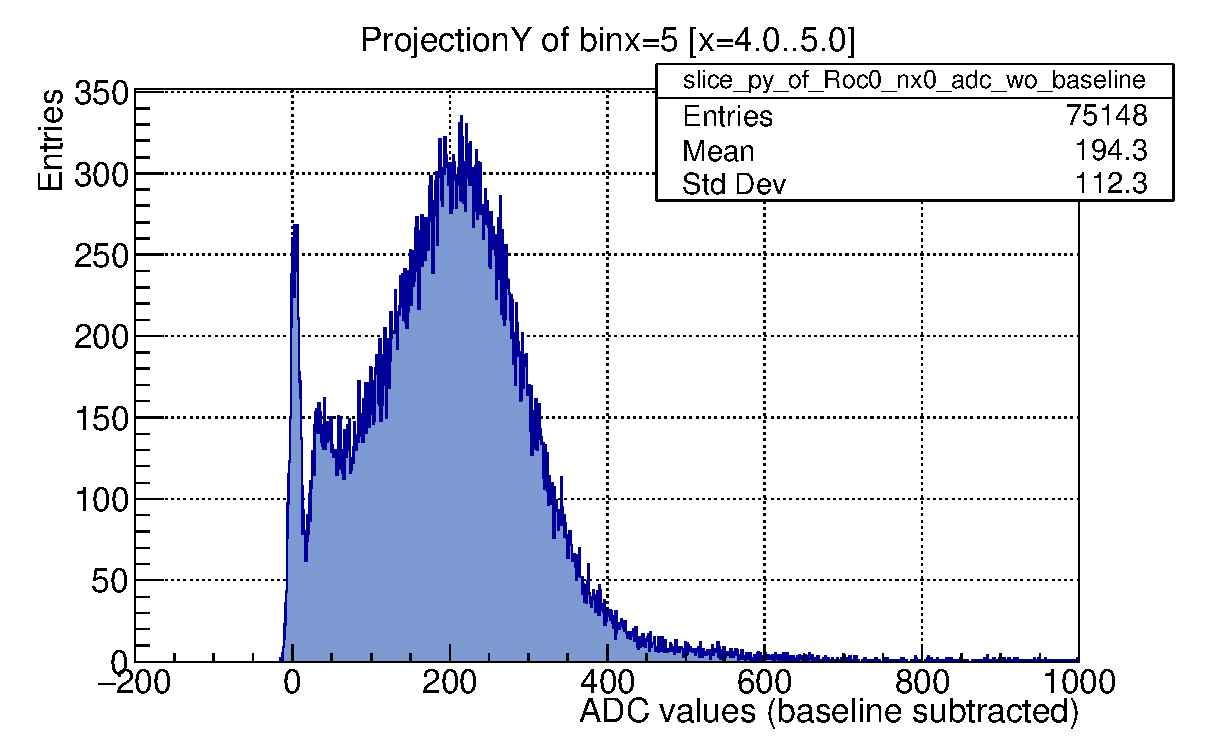
\includegraphics[width=1.0\textwidth]{pictures/PeculiarSpectrum.eps}
\caption{}
\label{fig:PeculiarSpectrum}
\end{figure}

Пик вблизи нуля соответствует наводке, возникающей в каналах, расположенных в одном ряду с тем, где зарегистрирован одноэлектронный сигнал. Двугорбое распределение справа соответствует настоящим одноэлектронным сигналам. Причем, левый пик связан с описанными в секции~\ref{section:secMapmt} событиями, когда электронная лавина или ее часть отклоняется от оптимального пути от динода к диноду. Отметим, что в большинстве каналов уровень шумов оказывается слишком высоким для отделения низкоамплитудного пика, связанного с наводкой от одноэлектронного сигнала. Таким образом, попытка получить максимальную эффективность регистрации за счет снижения порога приводит к возрастанию паразитных хитов, локализованных не в тех пикселях, где родился фотоэлектрон. Для снижения числа паразитных хитов мы ставили порог регистрации в ложбине между низко- и высоко-амплитудными частями одноэлектронного спектра. Поскольку формы одноэлектронных спектров во всех каналах подобны, анализ рисунка~\ref{fig:PeculiarSpectrum} позволяет заключить, что выбранный нами порог приводит к потере~???~\% одноэлектронных импульсов.

%пунктуация?
Одно из отличий канала считывания в плате PADIWA --- это значительно более быстрая, чем в n-XYTER аналоговая часть. Если в n-XYTER осуществляется формирование со временем интегрирования 190~нс, то в PADIWA происходит лишь подавление частот выше 100~МГц, что соответствует характерному времени нарастания сигнала несколько наносекунд. Такое отличие приводит к возрастанию роли быстрых шумов и наводок при регистрации сигналов с помощью PADIWA.

Информация о форме одноэлектронного спектра при считывании с помощью канала на основе плат PADIWA и TRB~v3 может быть получена в виде зависимости скорости счета событий вблизи триггера светового импульса от порога регистрации. Такие данные могут быть получены как из анализа потока даных, набранных при различных значениях порога, так и из значений счетчика зарегистрированых фронтов, реализованного непосредственно в ВЦП, упомянутого в секции~\ref{section:secModule}. При этом, использование счетчика позволяет достичь максимальных частот, достаточных для локализации базовой линии. На рис.~\ref{fig:TDCscalerScan} показана зависимость частоты триггеров в зависимости от порога регистрации. Плечо слева соответствует одноэлектронному спектру, а быстровозрастающие границы вблизи канала 34000 ограничивают локализацию базовой линии. Точность локализации базовой линии мы оцениваем как $ \pm $~??? отсчетов по шкале, использованной на рис.~\ref{fig:TDCscalerScan}.

%\begin{figure}
%\includegraphics[width=1.0\textwidth]{pictures/Thr_scan_flat.eps}
%\caption{Зависимость скорости счёта в одном канале от порога дискриминатора. Красная линия --- результат аппроксимации многочленом 7 степени.}
%\label{fig:ThrScan}
%\end{figure}

%\begin{figure}
%\includegraphics[width=1.0\textwidth]{pictures/Derivative_flat.eps}
%\caption{Аналитическая производная аппроксимирующей функции --- аналог одноэлектронного спектра.}
%\label{fig:ThrScanDeriv}
%\end{figure}

\begin{figure}
\includegraphics[width=1.0\textwidth]{pictures/TDCscalerScan.png}
\caption{}
\label{fig:TDCscalerScan}
\end{figure}

Результаты измерения частоты отсчетов, полученные с помощью счетчика и из анализа потока данных совпадают между собой, если полученное значение не превосходит *** при равномерной засветке всех каналов. (Совершенно не понятно, что это за предложение. Мы установили, что значения от этого счётчика совпадают со значениями, полученными анализом набранных данных. По-видимому, счётчик реально считает обработанные временные фронты, и если происходит затык из-за переизбытка фронтов, то и в данных и в счётчике будет спад, но одинаковый.)

Интересно сравнить зависимость скорости счета от порога при использовании двух систем считывания и одинаковых условиях засветки. Результаты такого сравнения для одного из типичных каналов показаны на рис.~\ref{fig:Blackboard}. В случае n-XYTER в таком сравнении может быть использован интеграл одноэлектонного спектра, показанный на рисунке~\ref{fig:Blackboard}a. Соответственно, производная указанной зависимости может быть сопоставлена с одноэлектронным спектром. Сплошная линия на рис.~\ref{fig:Blackboard}d получена дифференцированием кривой, показанной красным цветом на рис.~\ref{fig:Blackboard}b и полученной подгонкой измеренной зависимости полиномом 7-й степени. Отметим, что мы оцениваем равенство световых потоков как $ \pm $5\%. Видно, что скорости счета в области ложбины и максимума одноэлектронного спектра приблизительно совпадают. Амплитуды, соответствующие максимуму и ложбине соответственно, относятся как *** в обоих (или заметно отличие --- вряд ли, учитывая погрешность базовой линии!) случаях. При этом, в случае PADIWA наблюдается, с одной стороны более явно выраженная ложбина, а с другой --- избыток счета в малых амплитудах, что предполагает больший относительный вклад наводок и, следовательно, невозможность отделения от них низкоамплитудной части одноэлектронного спектра и нецелесообразность повышения эффективности за счет установления порога ниже ложбины.

\begin{figure}
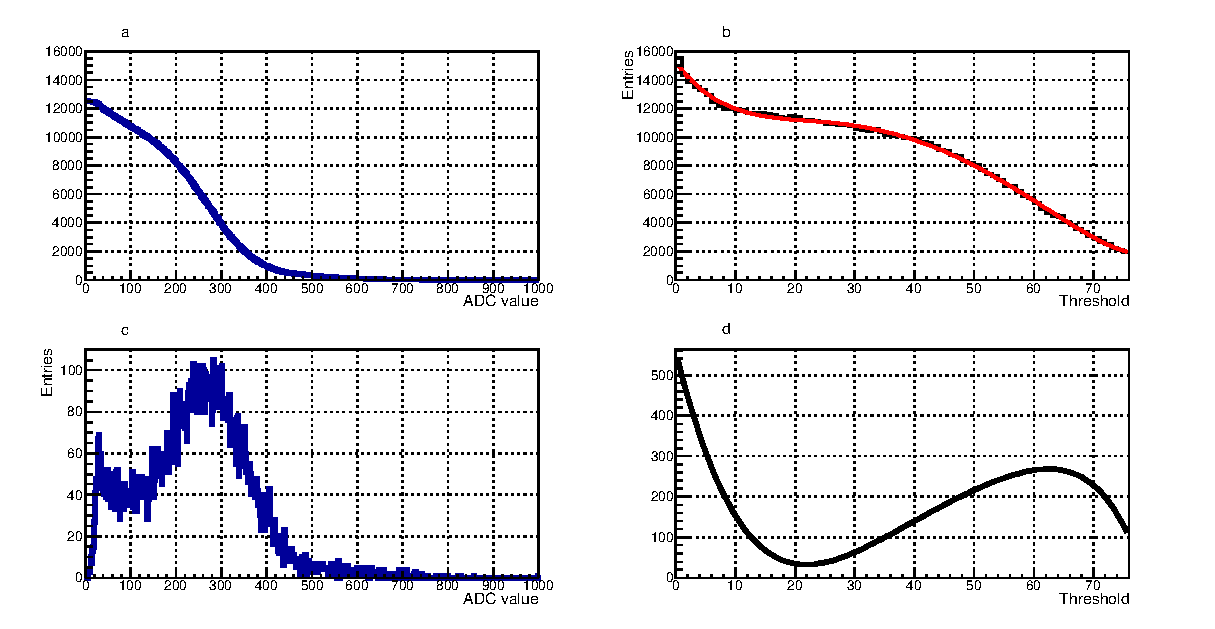
\includegraphics[width=1.0\textwidth]{pictures/Blackboard.eps}
\caption{}
\label{fig:Blackboard}
\end{figure}

